% remember to set these at the start of each chapter
\chapter{Experiments and Discussion} 

%%%%%%%%%%%%%%%%%%
\section{Dataset}
The dataset is obtained from western university. It contains 90 specimen samples, each of which has an Ultrasound (US) image stack and a Photoacoustic (PAT) image stack. The type of cancer (class) of each specimen is given in the dataset. The distribution of classes is 
{'B': 33, 'C': 21, 'A': 8, 'F': 6, 'E': 5, 'G': 5, 'H': 2, 'I': 2, 'K': 2, 'D': 1, 'L': 1, 'N': 1, 'J': 1, 'M': 1}.  
In this project, only class B and C are used. B has 33 samples and C has 21 samples. The other classes have too few samples to train a neural network on. 

For each image stack, US and PAT, the centre few images are extracted to use for training and testing. In a top-down scan of a specimen, the centre few images usually have the most detail and thus have most information of the specimen which work the best in classifying the specimen. An example of image stack is shown in Fig.\,\ref{stack}.

\begin{figure}[h]
	\centering
	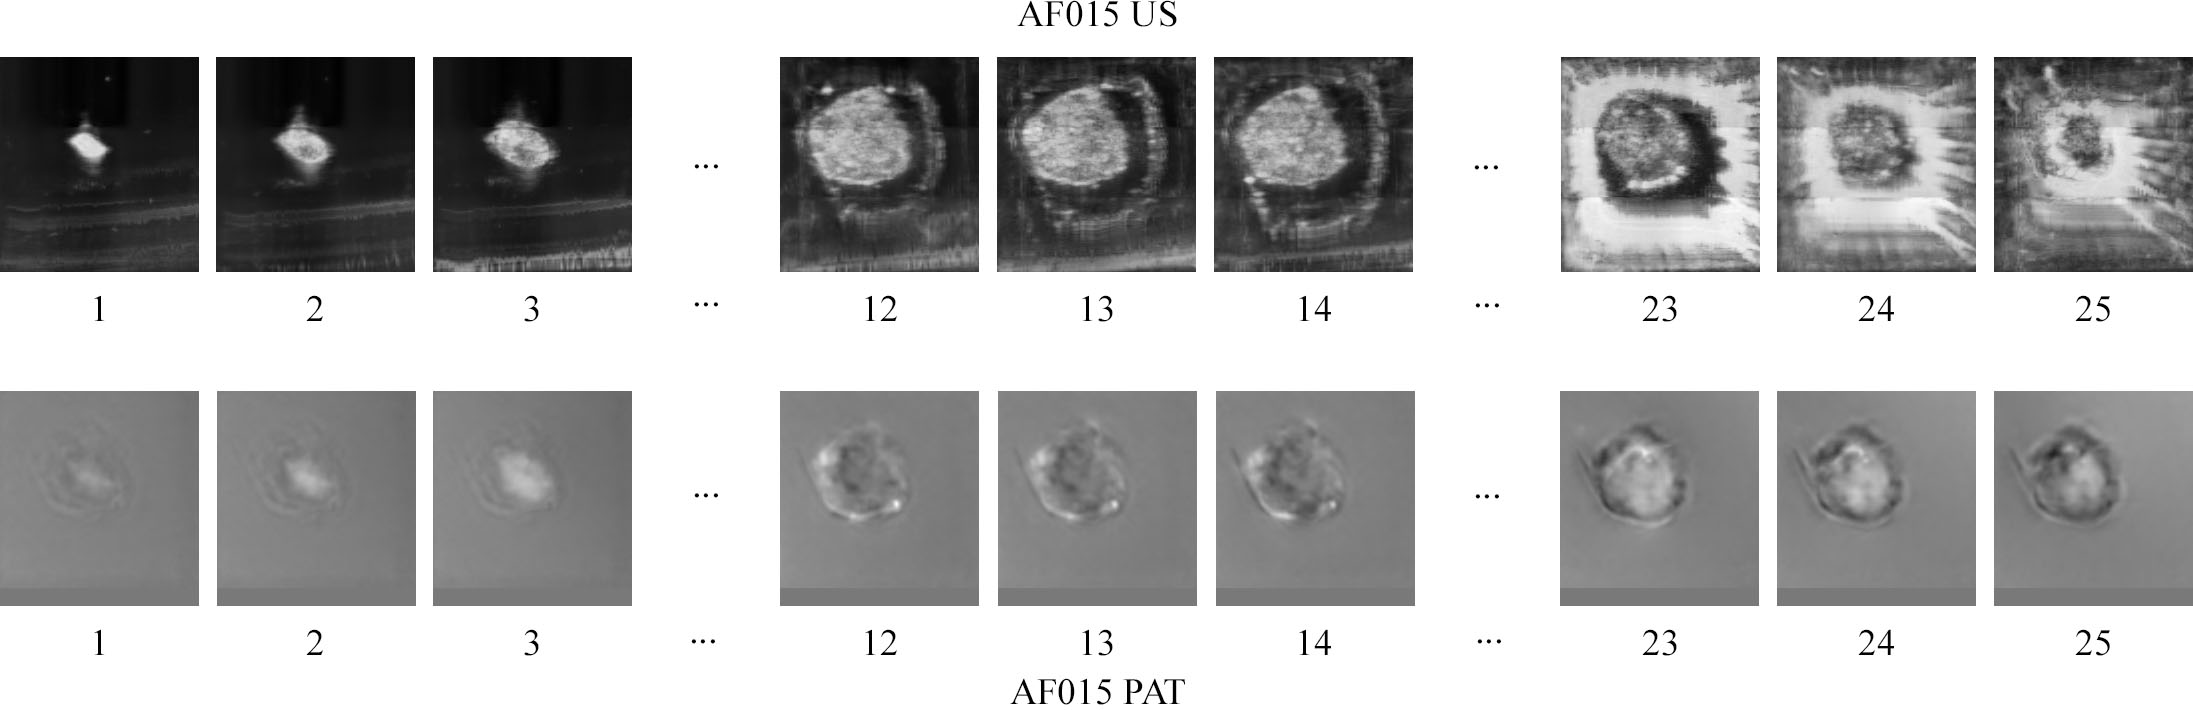
\includegraphics[width=\textwidth]{Figs/stack.jpg}
    \caption{US PAT stack example}
    \label{stack}
\end{figure}

We can see that the top few and bottom few scans have very low quality and lack of detail of the internal texture. The scans close to centre are larger in size and have the texture that classification could depend on.


\section{Data Partition and Augmentation}
The specimen samples are divided into training set and testing set by 0.8 ratio, 5-fold cross validation is used. Centre 6 images are extracted from a stack. No image from the same stack is separated into training and testing set. This is to ensure overfitting due to within-sample image similarities would not be possible. Because the number of samples in class B and C is not balanced, K-fold data partitioning is done by using Stratified k-fold. "StratifiedKFold is a variation of k-fold which returns stratified folds: each set contains approximately the same percentage of samples of each target class as the complete set". Each of the five folds is used as a test set once and only once. Accuracy and $F_1$ score is averaged across five folds.

Machine learning requires large amounts of data. While our dataset is very small, data augmentation is used to artificially expand the number of samples. Augmentation Scaling Factor is set to 5, meaning five images are created from one by Rotation, Cropping, Horizontal and Vertical Flip. Then, the images are resized to (200,200).

\section{Training}
"Adam" optimizer is used in all models to minimize the categorical cross-entropy across two classes. Adam is a replacement optimization algorithm for classic stochastic gradient descent. Adam can adaptively adjust the learning parameters based on the average first moment, as well as the average of the second moments of the gradients. The parameters of Adam optimizer is set to default. Training epoch is 50, all samples are passed to the network 50 times, with a batch size of 64. Best set of weights is saved. All parameters can be modified in YAML format for easier parameter fine tuning.


\section{Training Curves}

From the training curves, we can see that all training loss is decreasing and accuracy is increasing. However, the validation loss and accuracy is very noise, and do not have much improvement. Note that there is a large gap between training and validation curves. This indicates that the training dataset is unrepresentative, which means the training dataset does not provide sufficient information to learn the problem. We have too few examples in the dataset. From the noisy validation curves, we can conclude that the validation dataset is also unrepresentative. A  unrepresentative validation set means that it does not provide sufficient information to evaluate the ability of the model to generalize. This could occur when the validation dataset has too few examples.

\begin{figure}
\centering
\begin{subfigure}[b]{.3\linewidth}
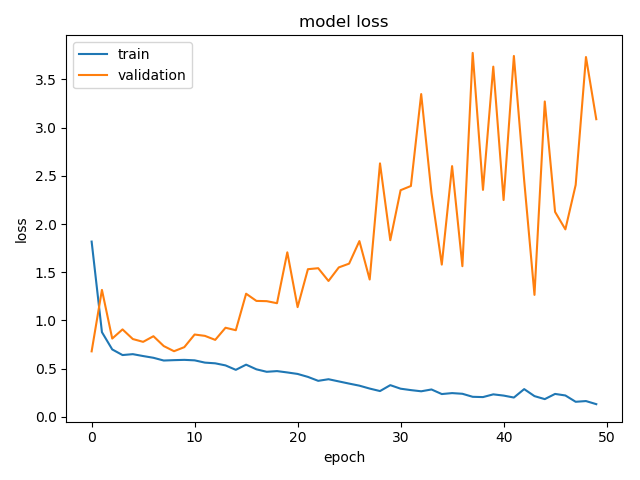
\includegraphics[width=\linewidth]{Figs/small_us_loss.jpg}
\caption{Small loss US}\label{fig:mouse}
\end{subfigure}
\begin{subfigure}[b]{.3\linewidth}
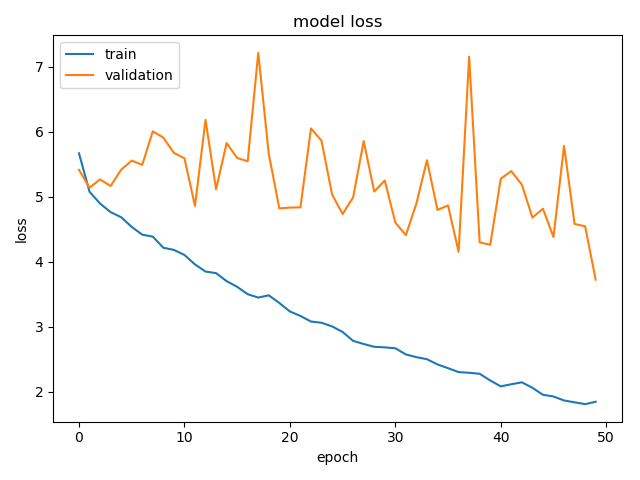
\includegraphics[width=\linewidth]{Figs/resnet_us_loss.jpg}
\caption{ResNet loss US}\label{fig:gull}
\end{subfigure}
\begin{subfigure}[b]{.3\linewidth}
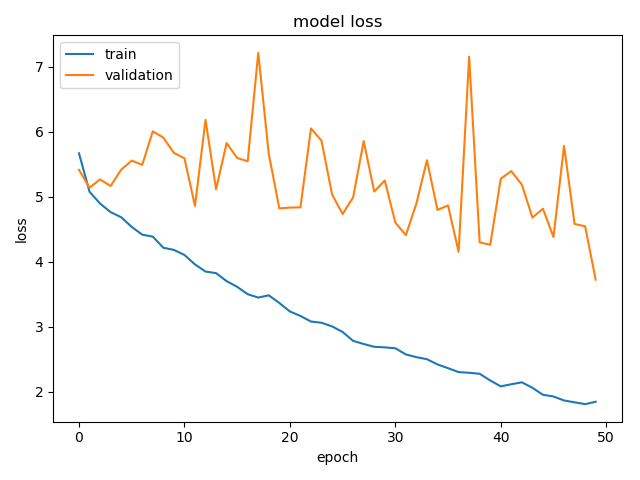
\includegraphics[width=\linewidth]{Figs/resnet_us_loss.jpg}
\caption{VGG loss US}\label{fig:tiger}
\end{subfigure}

\begin{subfigure}[b]{.3\linewidth}
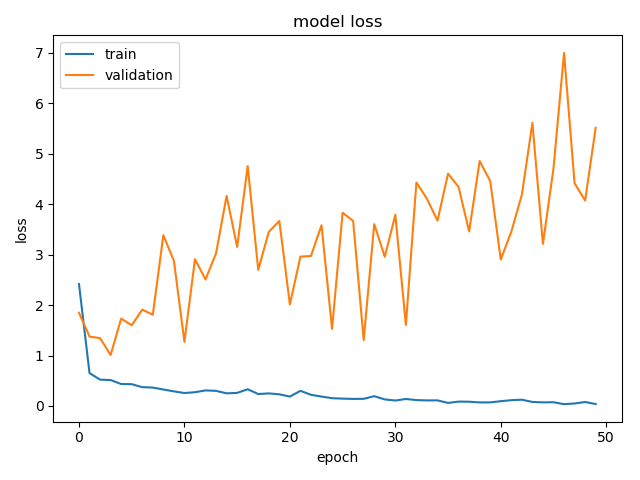
\includegraphics[width=\linewidth]{Figs/small_pat_loss.jpg}
\caption{Small loss PAT}\label{fig:tiger}
\end{subfigure}
\begin{subfigure}[b]{.3\linewidth}
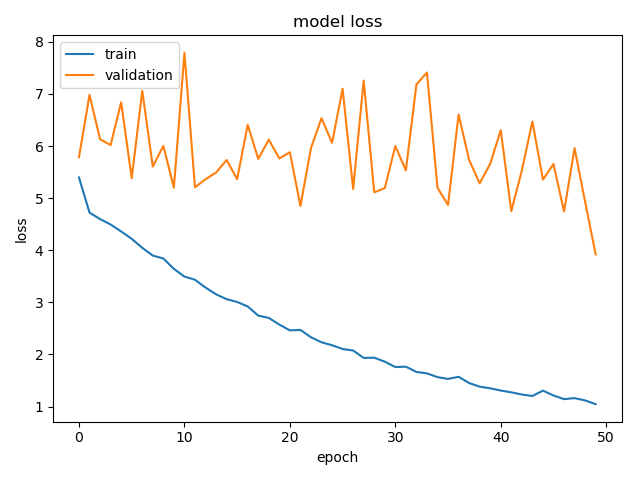
\includegraphics[width=\linewidth]{Figs/resnet_pat_loss.jpg}
\caption{ResNet loss PAT}\label{fig:tiger}
\end{subfigure}
\begin{subfigure}[b]{.3\linewidth}
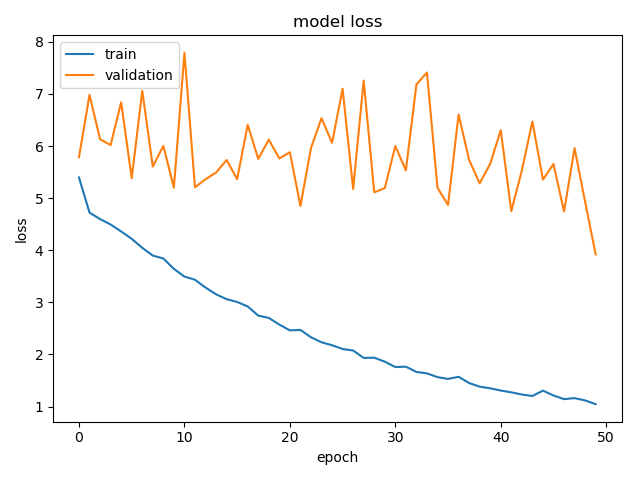
\includegraphics[width=\linewidth]{Figs/resnet_pat_loss.jpg}
\caption{VGG loss PAT}\label{fig:tiger}
\end{subfigure}
\caption{Model loss}
\label{fig:loss}
\end{figure}

\begin{figure}
\centering
\begin{subfigure}[b]{.3\linewidth}
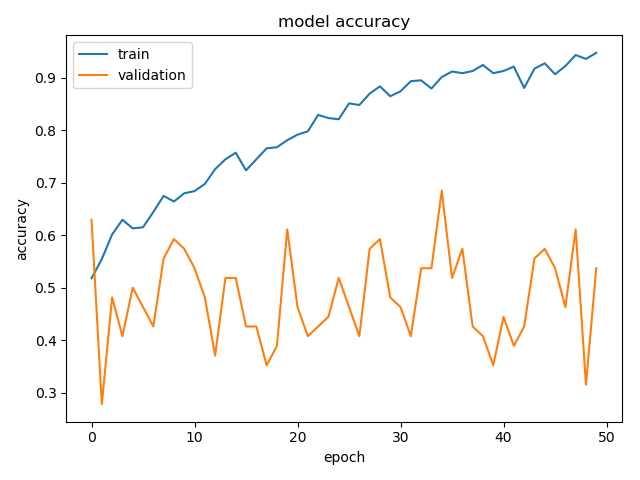
\includegraphics[width=\linewidth]{Figs/small_us_acc.jpg}
\caption{Small accuracy US}\label{fig:mouse}
\end{subfigure}
\begin{subfigure}[b]{.3\linewidth}
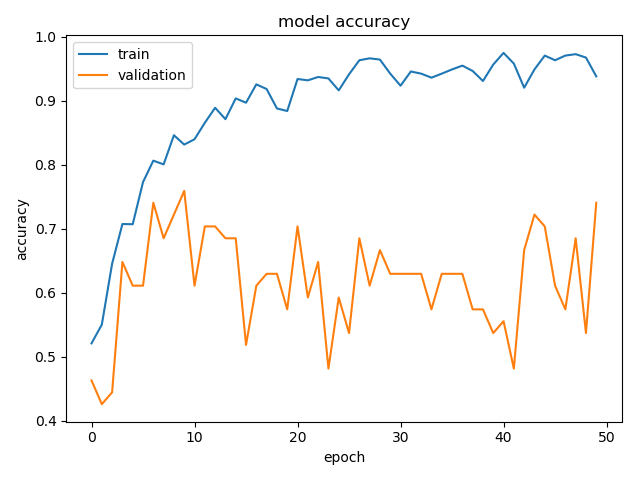
\includegraphics[width=\linewidth]{Figs/resnet_us_acc.jpg}
\caption{ResNet accuracy US}\label{fig:gull}
\end{subfigure}
\begin{subfigure}[b]{.3\linewidth}
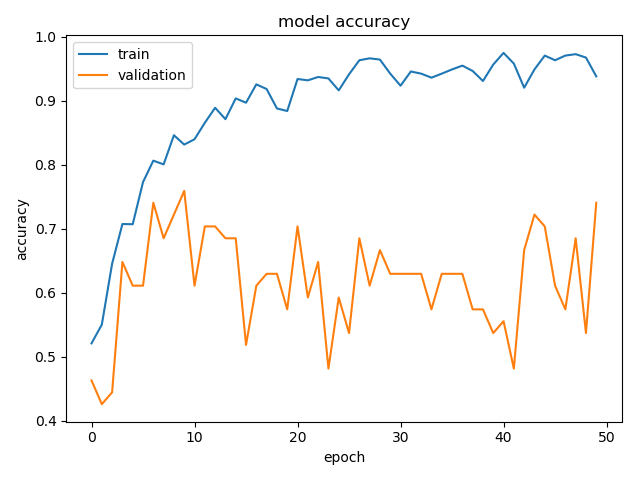
\includegraphics[width=\linewidth]{Figs/resnet_us_acc.jpg}
\caption{VGG accuracy US}\label{fig:tiger}
\end{subfigure}

\begin{subfigure}[b]{.3\linewidth}
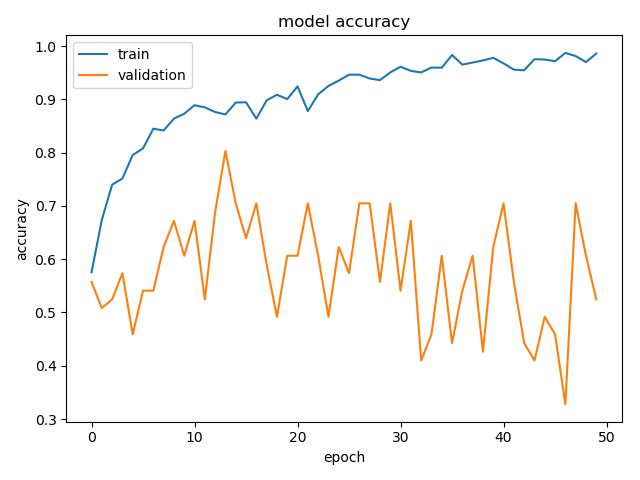
\includegraphics[width=\linewidth]{Figs/small_pat_acc.jpg}
\caption{Small accuracy PAT}\label{fig:tiger}
\end{subfigure}
\begin{subfigure}[b]{.3\linewidth}
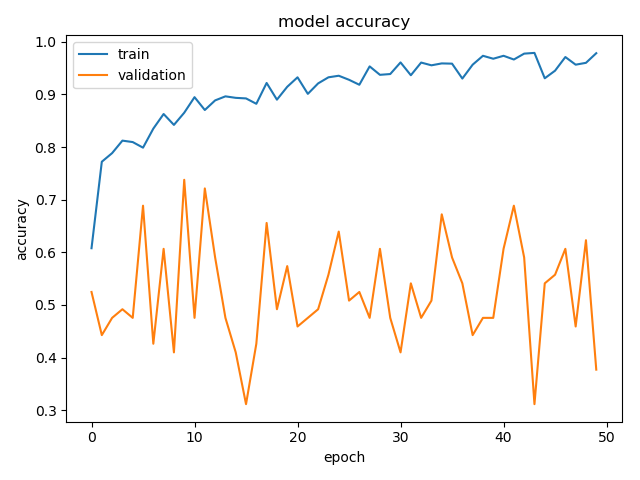
\includegraphics[width=\linewidth]{Figs/resnet_pat_acc.jpg}
\caption{ResNet accuracy PAT}\label{fig:tiger}
\end{subfigure}
\begin{subfigure}[b]{.3\linewidth}
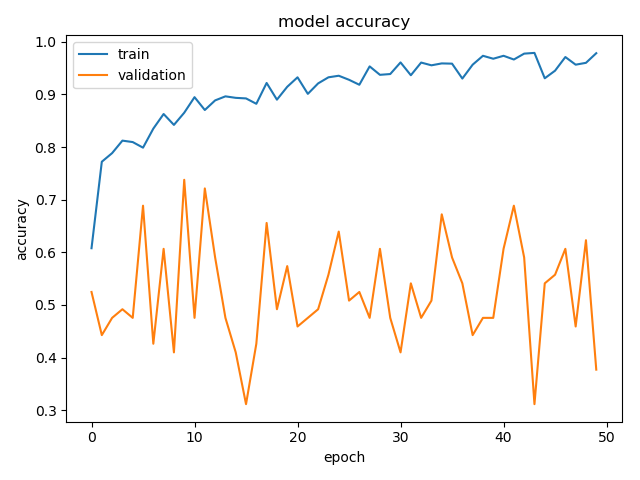
\includegraphics[width=\linewidth]{Figs/resnet_pat_acc.jpg}
\caption{VGG accuracy PAT}\label{fig:tiger}
\end{subfigure}
\caption{Model accracy}
\label{fig:loss}
\end{figure}



\section{Accuracy and $F_1$ score}
The $F_1$ score (also F-score) is a measure of a test's accuracy. It considers both the precision $p$ and the recall $r$ of the test to compute the score: $p$ is the number of correct positive results divided by the number of all positive results returned by the classifier, and $r$ is the number of correct positive results divided by the number of all relevant samples (all samples that should have been identified as positive). The $F_1$ score is the harmonic average of the precision and recall, where an $F_1$ score reaches its best value at 1 (perfect precision and recall) and worst at 0.
Formally: $$F_1 score = 2 \cdot \frac{precision \cdot recall}{precision + recall}$$
Presition $$p = \frac{TP}{TP + FP}$$
Recall $$r = \frac{TP}{TP + FN}$$
True Positives (TP): Samples which we predicted belong to a class, and they are indeed in the class.\\*
True Negatives (TN): Samples which we predicted not belong to a class, and they are indeed not in that class.\\*
False Positives (FP): We predicted in a class, but they are actually not.\\*
False Negatives (FN): We predicted not in a class, but they are actually in.\\*


\begin{table}[h]
\centering
\begin{tabular}{ |p{3cm}||p{3cm}|p{3cm}|p{3cm}|  }
 \hline
 Model       & Accuracy & Class B $F_1$ score & Class C $F_1$ score\\
 \hline
 Small  US   & 0.66  & 0.77 &  0.23\\
 ResNet US   & 0.75  & 0.82 &  0.55\\
 VGG US      & AL  & ALB &  008\\
 Small PAT   & 0.71  & 0.79 &  0.50\\
 ResNet PAT  & 0.76  & 0.83 &  0.57\\
 VGG PAT     & AD  & AND &  020\\
 \hline
\end{tabular}
\caption{Model accuracy and $F_1$ score}
\label{acctable}
\end{table}